\documentclass[a4paper,oneside,article,danish,table]{memoir}
\semiisopage \checkandfixthelayout
\XeTeXtracingfonts= 1
\usepackage{babel,microtype,verbatim,threeparttable,amsmath,amssymb,unicode-math,hyperref,siunitx,mhchem,tikz,pgfplots,tikz-timing}
\sisetup{per-mode=symbol}
\microtypesetup{final,verbose=silent}
\usetikzlibrary{mindmap,arrows,positioning,shapes}
%\setmainfont[Ligatures={TeX}]{Arno Pro}
\setmainfont{Linux Libertine O}
\setmathfont{[Asana-Math]}
%\hfuzz=1pt
\usepackage[margin,draft]{fixme}
\fxusetheme{color}

\newcommand{\authorvar}{Carl~Emil~Grøn~Christensen \& Mathias~Dannesbo}
\newcommand{\pretitlevar}{Teknikfag A eksamen:}
\newcommand{\titlevar}{Swagway} 
\newcommand{\subtitlevar}{0} 
\newcommand{\datevar}{\today} 
\newcommand{\subjectvar}{Teknikfag~A:~El}
\newcommand{\classvar}{}
\newcommand{\teachervar}{}

\makepagestyle{articlehead}
\makeevenhead{articlehead}{}{\titlevar}{}
\makeevenfoot{articlehead}{}{\thepage}{}
\makeoddhead{articlehead}{}{\titlevar}{}
\makeoddfoot{articlehead}{}{}{\thepage}
\pagestyle{articlehead}

\usepackage{listings,textcomp}
\lstset{language=[Visual]C++,
  morekeywords={[2]abs,acos,asin,atan,atan2,ceil,constrain,cos,degrees,exp,floor,log,map,max,min,radians,random,randomSeed,round,sin,sq,sqrt,tan,bitRead,bitWrite,bitSet,bitClear,bit,highByte,lowByte,analogReference,analogRead,analogWrite,attachInterrupt,detachInterrupt,delay,delayMicroseconds,digitalWrite,digitalRead,interrupts,millis,micros,noInterrupts,noTone,pinMode,pulseIn,shiftIn,shiftOut,tone,Serial,Serial1,Serial2,Serial3,begin,end,peek,read,print,println,available,flush,setTimeout,find,findUntil,parseInt,parseFloat,readBytes,readBytesUntil},
  keywordstyle={\bfseries\color[rgb]{0,0,1}},
  keywordstyle={[2]\bfseries\color[rgb]{0.8,0.33,0}},
  identifierstyle=\ttfamily,
  commentstyle=\color[rgb]{0.133,0.545,0.133},
  stringstyle=\color[rgb]{0.627,0.126,0.941},
  showstringspaces=false,
  basicstyle=\small\ttfamily,
  numberstyle=\footnotesize,
  numbers=left,
  stepnumber=1,
  numbersep=10pt,
  tabsize=2,
  breaklines=true,
  breakatwhitespace=false,
  upquote=true,
  extendedchars=true,
  literate={æ}{{\ae}}1
    {ø}{{\o}}1
    {å}{{\aa}}1
}

\newcommand{\boarddate}[1]{\textcolor{blue!80!black}{#1}}
\newcommand{\issue}[1]{\textsuperscript{\textcolor{blue!80!black}{\href{https://github.com/neic/Swagway/issues/#1}{\##1}}}}


\begin{document}
% \includepdf{forside.pdf} \clearpage%------------------------ Forside
\vfill
\noindent
{\fontsize{90}{108}\selectfont \color{red!80!black}\titlevar}\\
\color{blue!90!black}
{\LARGE \authorvar}\\
\datevar

\begin{center}
  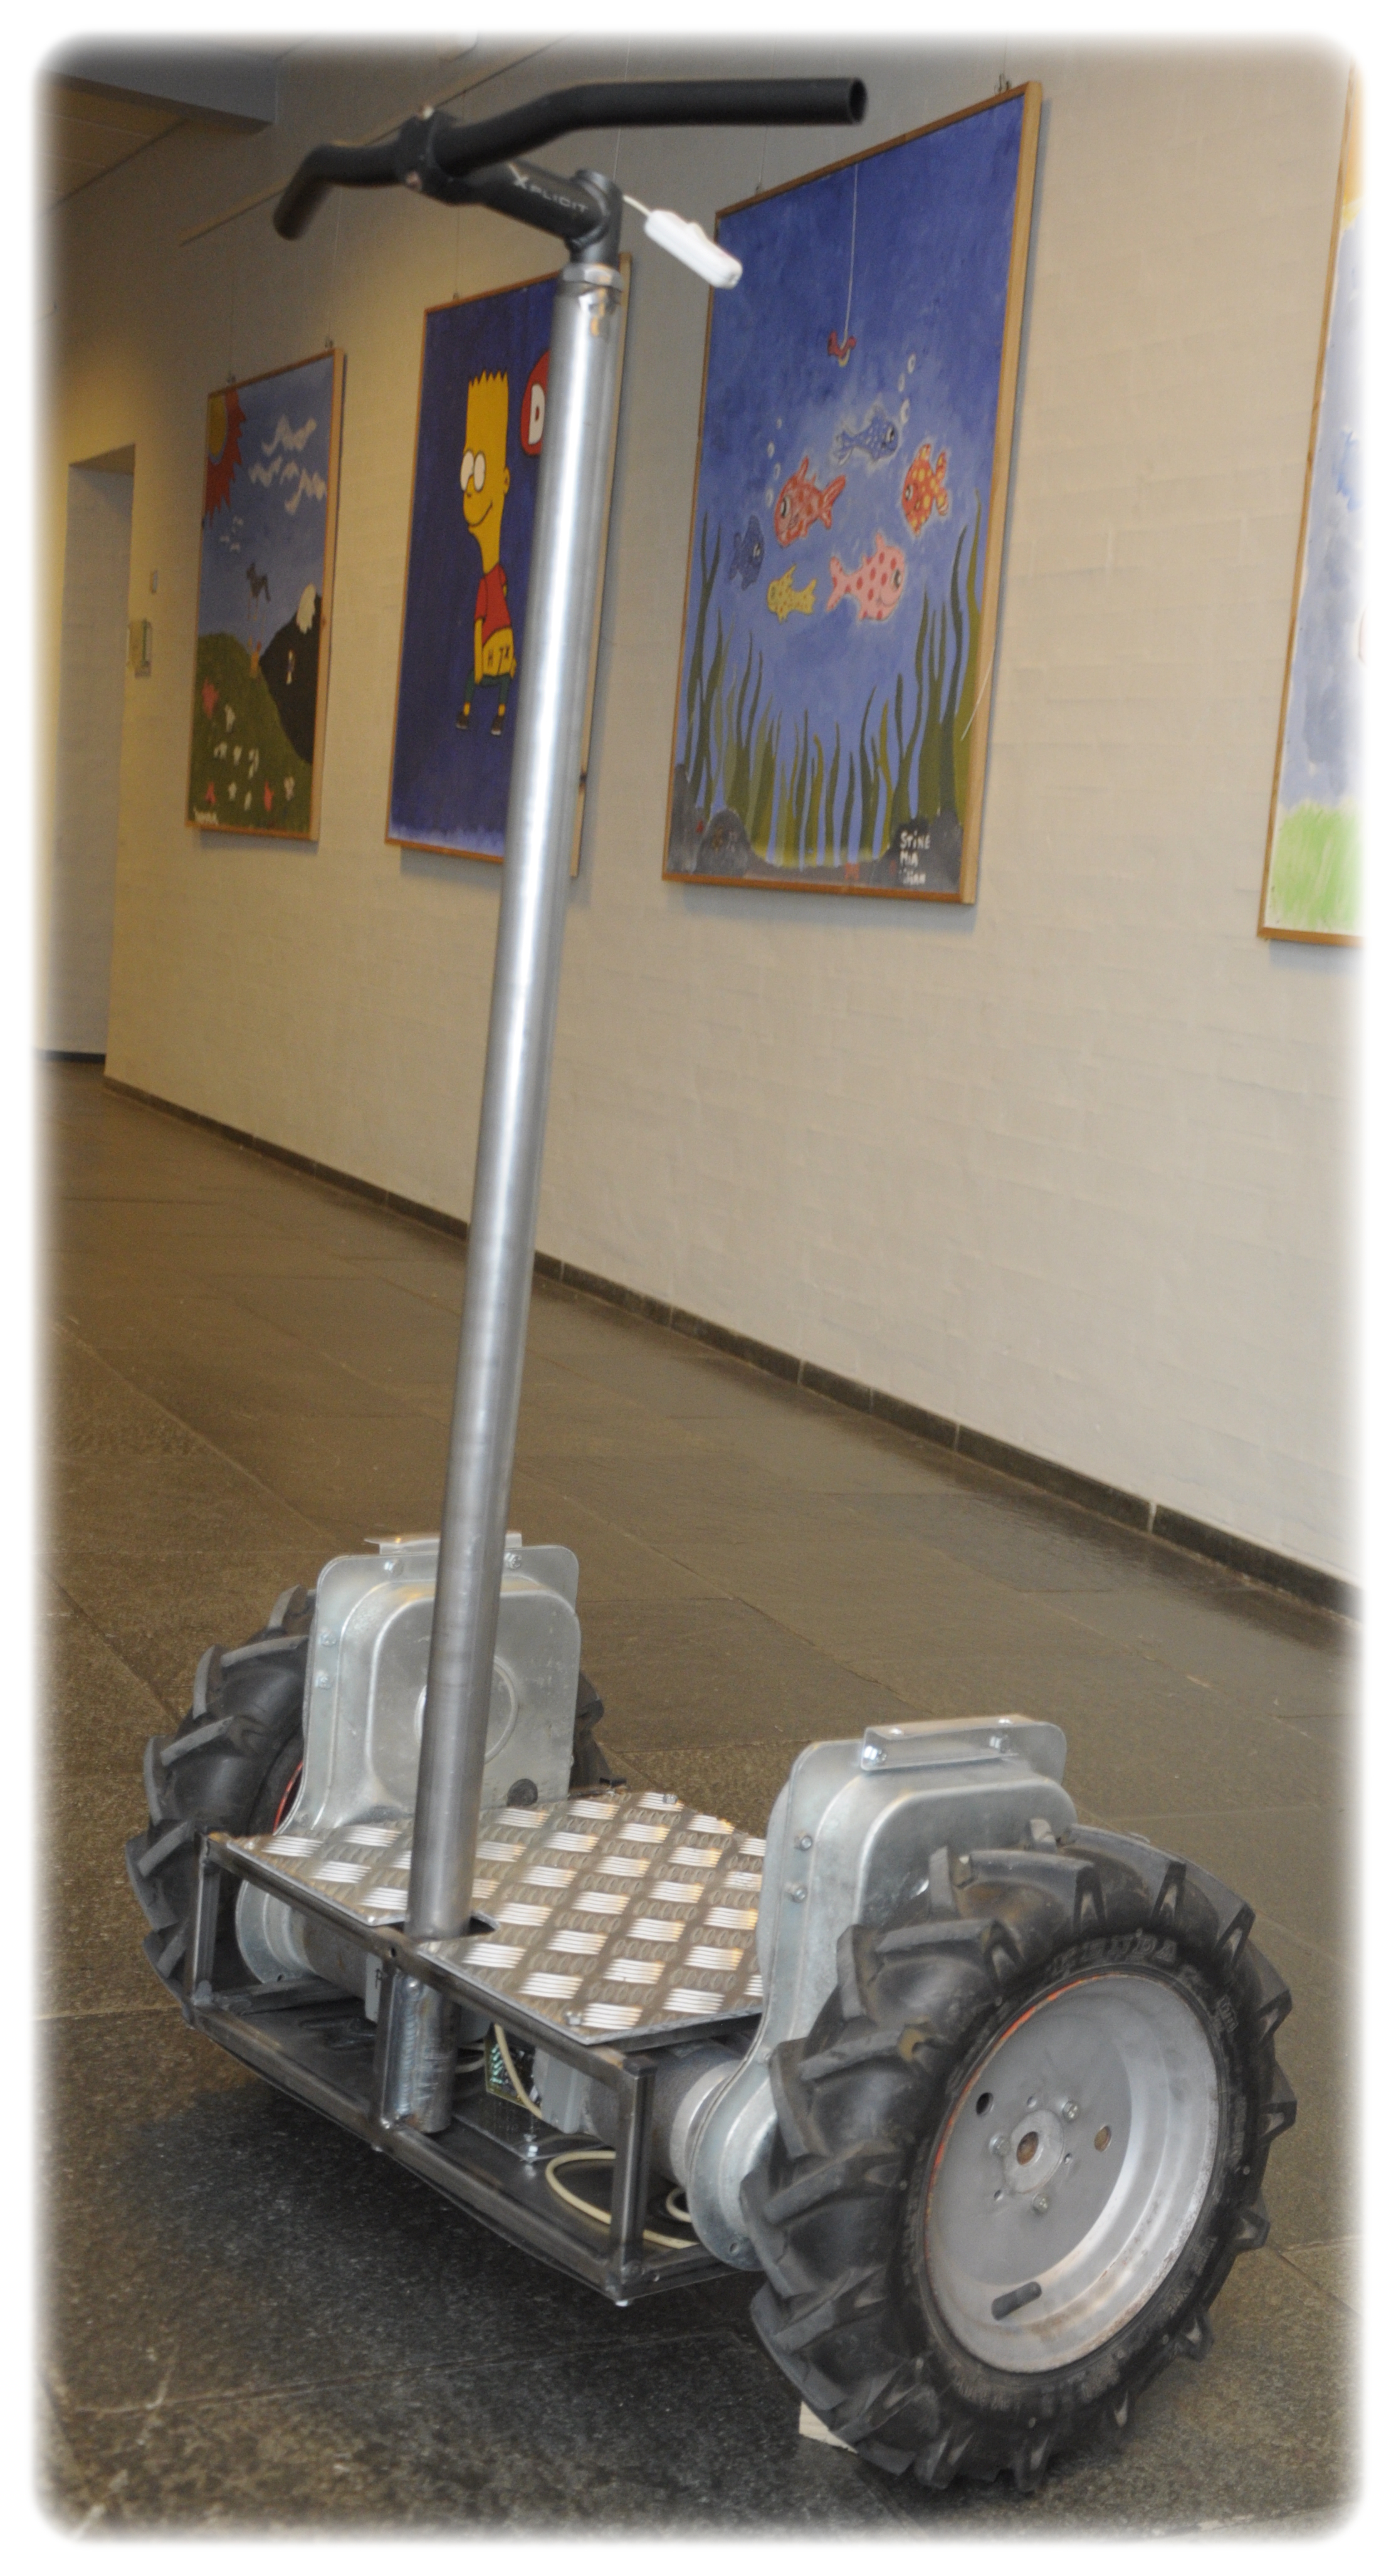
\includegraphics[width=0.3\textheight]{pictures/swagway.jpg}
\end{center}
\vfill
\thispagestyle{empty}
\clearpage
\begin{center}
  \if\pretitlevar 0
  \else{\Large\pretitlevar\\} \fi
  \textsc{\HUGE\titlevar\\}
  \if\subtitlevar 0
  \else {\Large\subtitlevar\\} \fi
  %\vspace{1em}
  {\LARGE 
  af\\
   \authorvar}\\
 \datevar\\
\end{center}

\vfill
\begin{abstract} %------------------------------ Abstract
  \fxwarning{Skriv resume}
\end{abstract}\vfill
\noindent
\begin{tabular*}{\textwidth}{@{\extracolsep{\fill}} ll}

\end{tabular*}
\thispagestyle{empty}
\clearpage

\chapter*{Forord}\label{chap:for}
Gennem teksten vil der være angivet link til “Issues” på GitHub siden for projektet.\footnote{\url{https://github.com/neic/Swagway}} Disse Issues har været brugt som projektstyring samt bugtracker igennem projektforløbet. Links er angivet som i enden af denne sætning.\issue{1} Det er ikke nødvendigt for forståelsen af denne rapport at følge linksne.

Vi vil gerne takke Steffen Linnerup Christiansen for hjælp med mekanikken, samt Kristian Holm Nielsen for hjælp med forståelsen af PID.

\clearpage \setcounter{tocdepth}{1} \tableofcontents \clearpage

\chapter{Indledning}\label{chap:ind}

Formålet med projektet er at bygge en motoriseret selvbalancrende tohjulet trasportenhed. Det er en klon af en Segway som er et komercielt produkt. Kendetegnet ved den er at de to hjul sidder på samme aksel. Elektronik og motorene sørger for at holde enheden lodret. Når en fører læner sig frem eller tilbage, kompenserer enheden ved køre i samme retning. For at dreje enheden vipper føreren håntaget til den side som man ønsker at dreje til.

Projektoplæget lyder:
\begin{quote}
  Formålet er at bygge en balance robot på to hjul, en Segway klon. Minimums målet er at få robotten til at balancere. Derefter få den til at køre og kunne styre den hvis tid og evner rækker til det.
\end{quote}

Hovedeudfordringen er at holde enheden lodret. For at gøre dette skal man kende enhedens vinkel i forhold til lodret og omsætte denne vinkel til et signal til motorene. Når vinklen stiger driver motorene hjulene som så flytter enheden og brugerens tygdepunk ind over akslen igen.
Det kan se som tre isolerede problemstillinger som passer ind i I-C-O-modellen:
\begin{itemize}
\item[Input] Mål vinklen.i forhold til lodret
\item[Control] Omsæt vinklen til et signal til motorene.
\item[Output] Driv to motore baseret på signalet.
\end{itemize}

\chapter{Input}

\section{Sensor}
Efter nogen research af andre køretøjer og mindre robotter med der fungere på sammen måde, var det klart at gyroskoper og accelerometere kunne måle vinklen så hurtigt og precist som det var krævet.

To sensorer, drift.
\subsection{Sensor hardware}
Pull-up, Bus capasistance, level shifter,

\subsubsection{Gyroskop}
Et gyroskop måler vinkelhastigheder, hvor hurtigt noget drejer om en akse. En normal 

. Hvis denne vinkelhastighed integreres over tid finder man vinklen gyroskopet har flyttet sig. Problemet med at integrer gyroskopdata er, at pga. måleusikkerheder vil det målte nulpunkt drive væk fra det fysiske nulpunkt.

\subsubsection{Accelerometer}
Et accelerometer kan måle accelerationer. Man kan med hjælp fra tangens og data fra to akser udregne den vinklen accelerometeret står i forhold til jordens tyngdekræft. Problemet med dette er at accelerometer måler alle accelerationer, ikke kun jordens tyngdekræft. Når Swagwayen fx accelerer, bremser eller køre over en sten bliver den udregnet vinkel forkert.

%For at komme begge problemer til livs bliver begge sensorer brugt og data fra begge to bliver samlet i et såkaldt Kalman-filter. Kalman-filtret kan tilnærmelsesvis ses som et high-pass og low-pass filter. Det taget de hurtige ændringer (high-pass) fra gyroskop-dataene og bruger accelerometer-dataene til at holde det målte og det fysiske nulpunkt ens.

\begin{figure}[htbp]
  \centering
  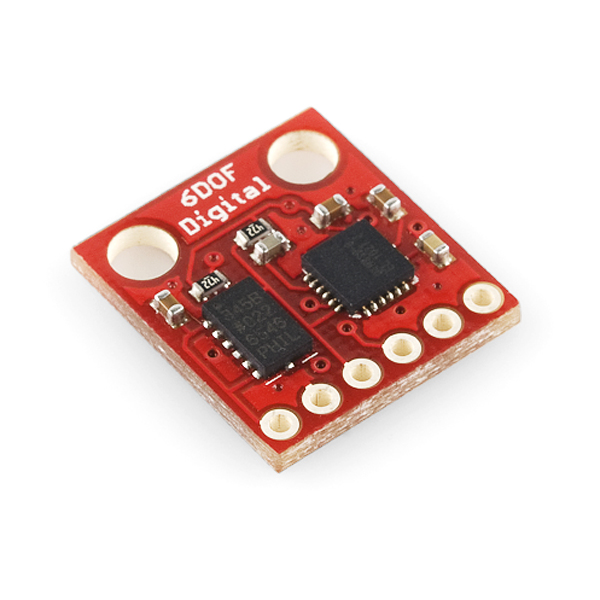
\includegraphics[width=0.3\textwidth]{pictures/imu.jpg}
  \caption[IMU breakoutboard fra Sparkfun]{IMU breakoutboard fra Sparkfun. (CC BY-NC-SA 3.0, Sparkfun)}
  \label{fig:imu}
\end{figure}
\subsection{Sensor software}
I²C, wire.h, libraries

IMUen kører på I²C bussen som blev skabt af Philips for mange år siden, og bliver brugt mellem en eller flere "masters", som i vores tilfælde er Arduinoen, og en eller flere "slaves", eks. IMUen. I²C bussen består af to fysiske wires, en serial data line (SDA) og en serial clock line (SCL). 
Masteren er den enhed som bestemmer Standard Clock Line, og slaverne er den enhed som lystrer til masteren. Hastigheden på forbindelsen kan være 100KHz, 400KHz eller 3400KHz. Masteren er den eneste som kan starte en forbindelse mellem enhederne, og det gør den ved at starte en sekvens på bussen, som ændrer SDA fra høj til lav. Start sekvensen indikerer i en bit, om masteren vil modtage data fra slaven, eller om den vil sende til slaven. Denne bit, også kaldet LSB eller Least Significant Bit placeres efter syv andre bits, som er slavens adresse. Herefter udsendes endnu en bit, som slaven skal besvare ved at trække SDA lav. Denne bit kaldes ACK som står for acknowledgement, som betyder anerkendelse. Herefter sendes der data via. SDA synkront med clock linen, som afsluttes med endnnu en ACK bit. Til slut skiftes SDA til høj igen, mens SCL beholds høj.  
\section{Styring}
Mål: En længerevarende og holdbar løsning til at styre Swagwayens retning.
Potentiometer, gaffelsensor, strain-gate

\chapter{Control}
\section{Filter}
Mål: At samle data fra gyroskop og accelerometer og regne en vinkel ud

Målet med filtret er at samle dataen fra gyroskopet, accelerometeret og ud fra disse beregne en vinkel, som vi kan benytte til at regulere PWM efter. Ud fra dette mål, udvalgte vi tre filtre, som har de egenskaber vi leder efter.
\subsection{Komplementær filter}
\subsection{Kalman filter}
\subsection{Modificeret Kalman filter}

\section{Regulering}
Mål: At omsætte en vinklen til en PWM værdi.

For at kontrolere hvorledes Swagwayens motorer bevæger sig i forhold btil vinklen, skal vi bestemme et forhold mellem vinklens hældning og PWM. 
\subsection{Lineær}
\subsection{PID}
\subsection{Eksponentiel}

\chapter{Output}
Mål: At køre motorene i begge retninger med variabel hastighed.
\section{H-broens virkemåde}
H-bro teori
\section{PWM}
Pulsbreddemodulation (Pulse-Width-Modulation): Er en metode til at kontrollere spændingen i elektriske
apparater. Det er en metode til at levere spænding igennem en række impulser i stedet for der konstant er strøm igennem systemet. Ved at øge eller formindske bredden af impulsen kan man kontrollere en motor.

Man kan altså sige, at PWM er et on/off system hvor man styrer ved hurtigt, at slukke og tænde for
spændingen. Tiden der går imellem at den er on/off er så kort, at en LED som sådan ikke mærker det. Så
den vil ikke blinke, men derimod lyse mindre hvis man øger bredden imellem impulserne.

Måden vi styre dette på i en Arduino er via \texttt{analogWrite(pin,\dots);}. Her har vi mulighed for at give en værdi fra 0--255. Dette betyder at \texttt{analogWrite(pin,255);} er 100\% og \texttt{analogWrite(pin,127);} er 50\%. Dette kan også ses på figur \ref{fig:pwm}.\fxwarning{Hele afsnittet skal omskrives}
\begin{figure}[htbp]
  \centering
  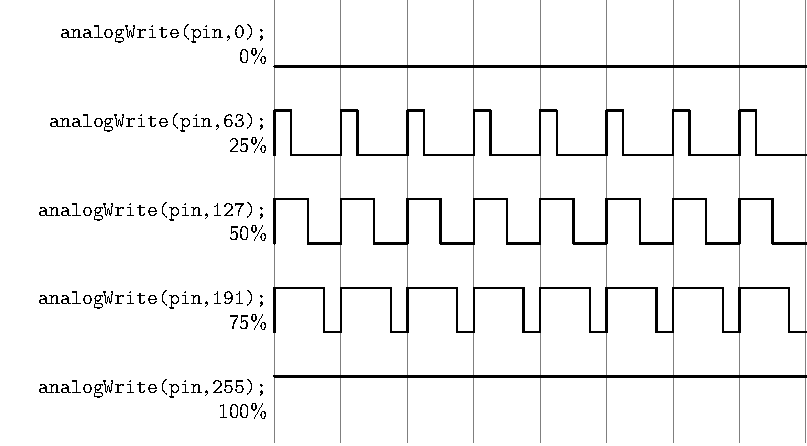
\includegraphics[width=\textwidth]{pictures/pwm.pdf}
  \caption{Eksempel på PWM med varierende dutycycle}
  \label{fig:pwm}
\end{figure}

\section{Overvejelser}
Vores valg: Dobbelt H-bro med mange chip eller bygge selv. Med eller uden PWM “i bunden”.
\section{Motorcontroller}

\begin{table}[htbp]
  \caption{Motorcontroller v5.2 sandhedstabel}
  \centering
  % \begin{threeparttable}
  \begin{tabular}{ccc|cccc|ccccl}
    \toprule
    \multicolumn{3}{c}{Arduino pin}&\multicolumn{4}{c}{HEXFET spænding}&\multicolumn{4}{c}{HEXFET on/off}\\
    P7&P6&P5 &Q1&Q2&Q3&Q4 &Q1&Q2&Q3&Q4\\
    P8&P9&P10 &Q5&Q6&Q7&Q8 &Q5&Q6&Q7&Q8\\
    \midrule
    0&0&0 &0&1&0&0 &0&0&0&1 & Off ($\circlearrowright$)\\
    1&0&0 &0&0&0&1 &0&1&0&0 & Off ($\circlearrowleft$)\\
    0&1&0 &1&1&0&0 &1&0&0&1 & $\circlearrowright$\\
    1&1&0 &1&0&0&1 &1&1&0&0 & Short\\
    0&0&1 &0&1&1&0 &0&0&1&1 & Short\\
    1&0&1 &0&0&1&1 &0&1&1&0 & $\circlearrowleft$\\
    0&1&1 &1&1&1&0 &1&0&1&1 & Short\\
    1&1&1 &1&0&1&1 &1&1&1&0 & Short\\
    \bottomrule
  \end{tabular}
  % \begin{tablenotes}
  % \end{tablenotes}
  % \end{threeparttable}
  \legend{Tabellen viser hvordan den seneste motorcontroller, v5.2, opføre sig hvis den får inputtet angivet under “Arduino Pin”}
  \label{tab:sandhed}
\end{table}

H-bro, PWM, PWM-kondensator, beskyttelses dioder, 4000 serie, optocopler

\subsection{Samlet board}
Det var upraktisk at have alle funktioner på samme board. H-broerne og optocouplerne blev flyttet på sit eget board “Motorcontroller v1.0”.

\subsection{Motorcontroller v1.0}
\boarddate{24. januar 2012}
\fxwarning{Indsæt diagram over Motorcontroller v1.0}
\fxwarning{Indsæt figur over Motorcontroller v1.0}
Boardet virkede ikke. Det opførte sig som det var kortsluttet. Det viste sig, at efter boardet var skilt helt af igen, at det plus tegn der skulle vise polariteten var sat ved den forkerte pol. Printet havde taget skade af at blive loddet på flere gange.

Der var desuden nogle af ledningene for tætsiddene og loddeøerne var lidt underdimensionerede. Der manglede også en mulighed for at se, hvilken vej strømmen løber i H-broerne. Dette blev rettet i v2.0.
\subsection{Motorcontroller v2.0}
\boarddate{8. marts 2012} Dette board blev aldrig lavet færdigt; Ledningerne omkring pinheaderen var for tæt efter at loddeøeren blev forstørret. Diagram og figur over printet kan findes i bilag. \fxwarning{ref}

\subsection{Motorcontroller v2.1}
\boarddate{8 marts 2012}
\begin{figure}[htbp]
  \centering
  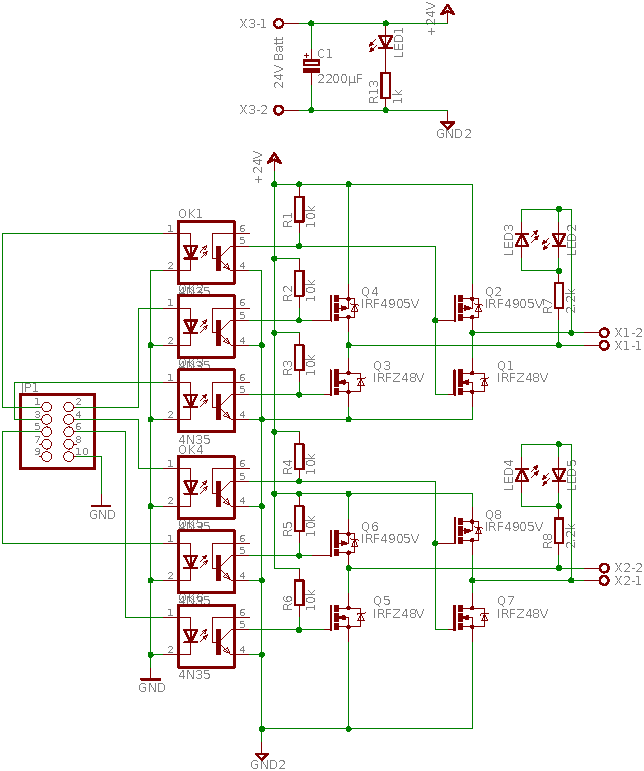
\includegraphics[width=\textwidth]{pictures/MotorcontrollerSch2-1.pdf}
  \caption{Diagram over Motorcontroller v2.1}
  \label{fig:mosch2.1}
\end{figure}

\fxwarning{ref til fig:mosch2.1}

Boardet fungerede umiddelbart. Motoren kunne køre i begge retninger og farten kunne styres med PWM. Dog startede motoren på ca. 30\% fart i den ene retning. Ved at måle på PWM signalet fra mainboardet og signalet til motoren kunne problemet indskrænkes til at være på Motorcontrolleren.

Det viste sig efter megen debugging, at spændingen på gaten på P-kanal HEXFETerne (IRF4905) ikke gik \texttt{HIGH} lige så hurtigt som forventet. Der blev opstillet et forsøg på et breadboard med en P-kanal HEXFET, en optocoupler og en Arduino.

\fxwarning{Indsæt diagram over forsøg med optocoupler og HEXFET}

Forsøget viste, at når optocoupleren sad mellem HEXFETen og Arduinoen var der en kapacitet mellem HEXFETens gate og source. Figur \ref{fig:stigetid} viser nederst PWM signalet fra Arduinoen og øverst signalet på P-kanal HTXFETens gate. Man ser tydeligt at det tager en ubelejlig tid før signalet på gaten stiger.
\begin{figure}[htbp]
  \centering
  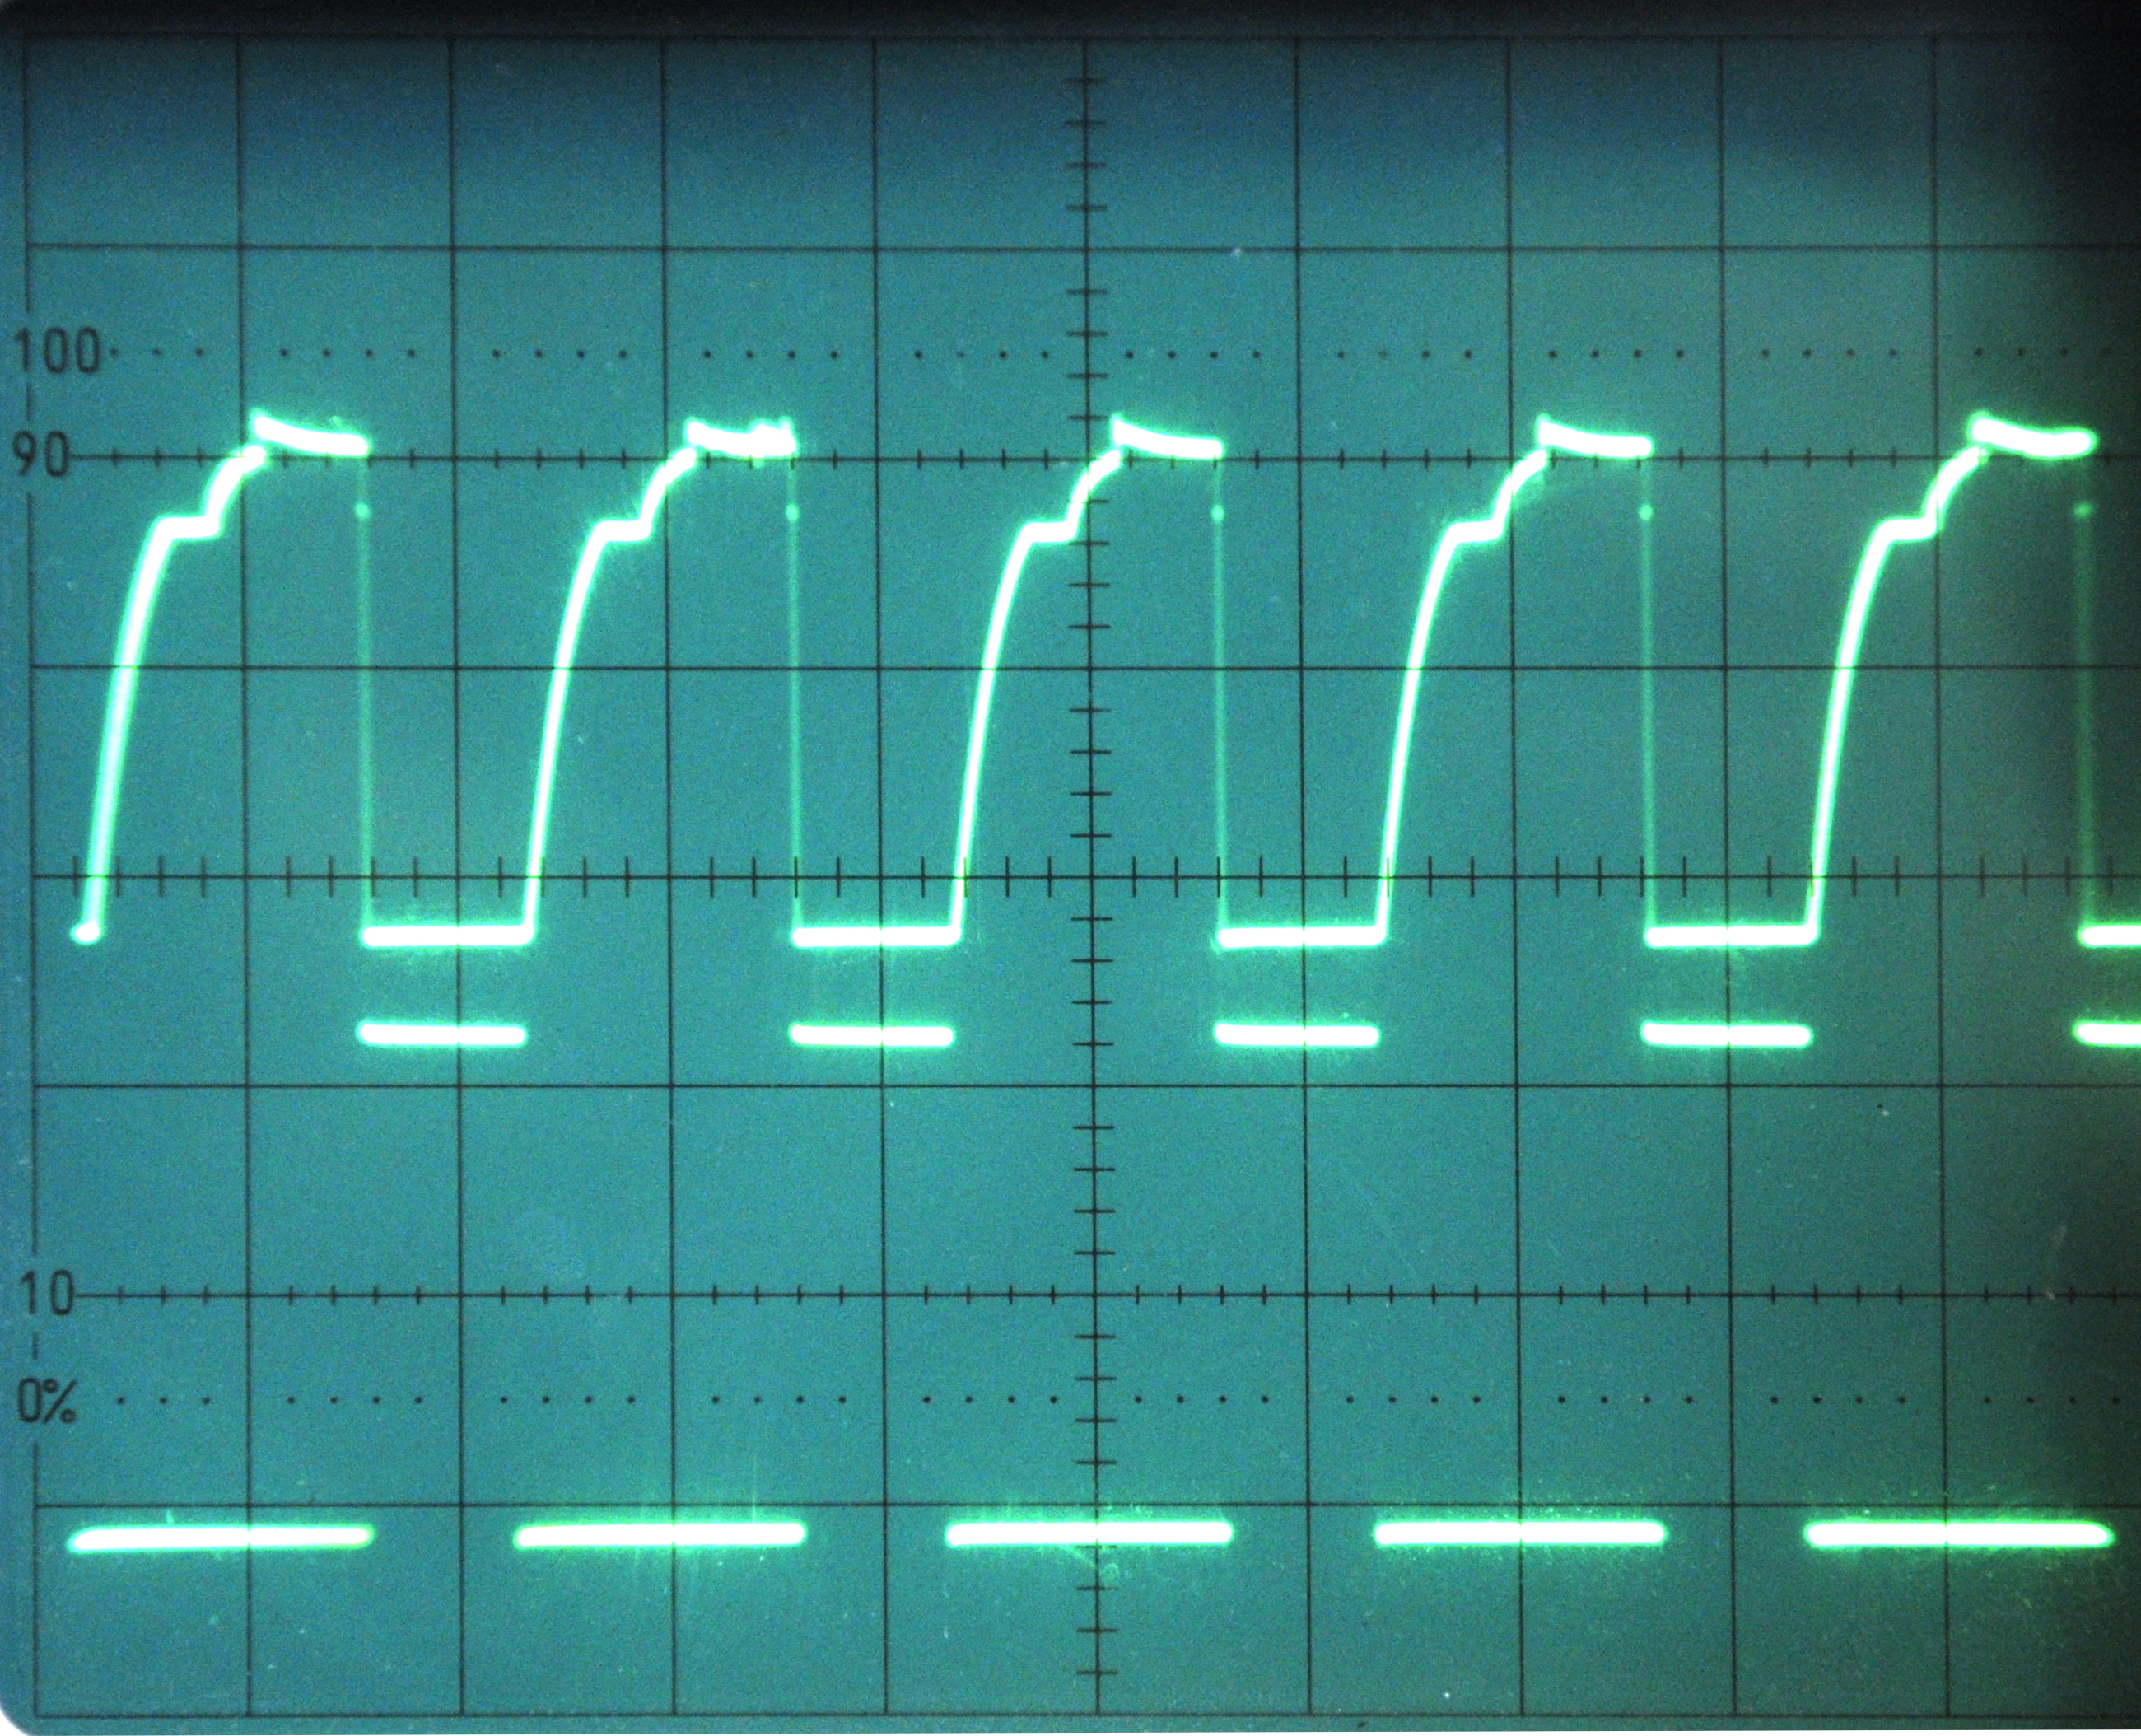
\includegraphics[width=0.8\textwidth]{pictures/stigetid.jpg}
  \caption[Oscilloskop billede af stigetid på en P-kanal HEXFET gate]{Oscilloskop billede af stigetid på en P-kanal HEXFET gate. Nederst ses PWM-signalet fra Arduinoen, øverst ses signalet på gaten.}
  \label{fig:stigetid}
\end{figure}

Ved at sætte en mindre pull-up-modstand på kunne den aflades hurtigere, men det var ikke muligt at få den tilpas langt ned til at kunne styre motoren godt. Ved at fjerne optocoupler og køre HEXFETens gate direkte fra Arduinoen eller ved fjerne HEXFETen og måle direkte på optocoupleren, var stigningstiden $\approx0$. Det var kun i kombination mellem HEXFETen og transistoren i optocoupleren at stigningstiden ikke var $\approx0$.

Der blev forsøgt med en 4N25 optocoupler istedet for 4N35 og en BC547 istedet for optocoupleren; der var samme stigningstid.

Det har ikke været muligt, selv med hjælp fra vejleder, at forklare hvorfor denne kapacitet er der.

Problemet blev ikke løst, det blev bare gjort ubetydeligt: Istedet for at bruge en N- og en P-kanal HEXFET til at bestemme retning og køre PWM på de andre to N- og P-kanal HEXFETer, blev det lavet om til at begge P-kanal HEXFETer blev brugt til at bestemme retning og at N-kanal HEXFETerne bliver brugt at køre PWM. Det er ikke et problem at stigetiden på P-kanal HEXFETerne er langsom da de kun ændre sig når der skiftes retning og ikke med høj frekvens som ved PWM.

For ikke at tilføje flere optocouplere og bruge flere pins på arduinoen blev der, på Motorcontrolleren tilføjet to invertere. Se figur \fxwarning{ref: dia:v3.0}
\subsection{Motorcontroller v3.0}
\boarddate{27. marts 2012}
\fxwarning{Indset diagram over Motorcontroller v3.0 (Figur over printet kan findes i bilag)}
Efter at der blev tilføjet en inverter på to af gatesne til P-kanal HEXFETerne er denne low når der ikke er spænding på optocouplerne (fx når den ikke er koblet til Mainboardet). Det tænder HEXFETen, det, sammen med N-kanal HEXFETerne som også er tændt uden spænding på optocouplerne, kortslutter H-broen. Motorcontroller v3.0 var fungerede, men det var upraktisk at den var kortsluttet unden at være koblet sammen med Mainboardet.

Pull-up modstandende blev erstattet af pull-down.
\subsection{Motorcontroller v4.0}
\boarddate{12. april 2012} Dette board blev aldrig lavet færdigt. En stor del af boardet blev re-routed da der var blevet rodet efter mange versioner. Diagram og Figur over printet kan findes i bilag. \fxwarning{ref}

\subsection{Motorcontroller v4.1}
\boarddate{13. april 2012}
Der var en ledning der ikke var routed og der var noget mindre re-routing.

\subsection{Motorcontroller v4.2}
\boarddate{17. april 2012} Dette board blev aldrig lavet færdigt.
Formodstandene til optocouplerne blev flyttet fra mainboardet til Motorcontrolleren, for at undgå, at disse blev brændt af.

\subsection{Motorcontroller v5.0}
\boarddate{24. april 2012} Dette board blev aldrig lavet færdigt.
Der blev tilføjet LEDer til optocouplerne så man kan se hvornår de er tændt, og for at lette debugging.  

\subsection{Motorcontroller v5.1}
\boarddate{24. april 2012} Dette board blev aldrig lavet færdigt.
Nogle pins blev flyttet i fladkablet. 

\subsection{Motorcontroller v5.2}
\boarddate{24. april 2012}
\fxwarning{Board brænder af}
\begin{figure}[htbp]
  \centering
  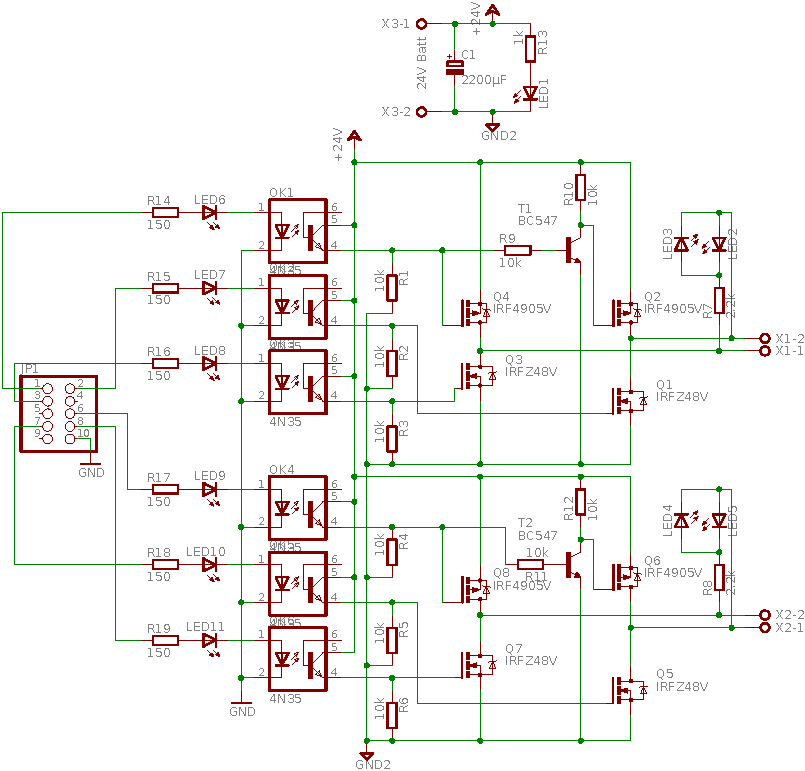
\includegraphics[width=\textwidth]{pictures/MotorcontrollerSch5-2.pdf}
  \caption{Diagram over Motorcontroller v5.2}
  \label{fig:mosch5.2}
\end{figure}
\fxwarning{ref til fig:mosch5.2}

Dette board fungerer og sidder i Swagwayen.

\subsection{Motorcontroller v6.0}
\boarddate{24. april 2012}

\chapter{Auxiliary}
\begin{table}[htbp]
  \caption{Pin forbindelser på Arduino}
  \centering
  \begin{threeparttable}
    \begin{tabular}{rll}
      \toprule
      Pin & Forbindelse & Egenskaber\\
      \midrule
      0 & USB Rx & \\
      1 & USB Tx & \\
      2 & Radio Rx & Interrupt\\
      3 & & Interrupt, PWM\\
      4 & Radio Tx & \\
      5 & Motorcontroller R2 & PWM\tnote{a}\\
      6 & Motorcontroller L2 & PWM\tnote{a}\\
      7 & Motorcontroller L1 & \\
      8 & Motorcontroller R1 & \\
      9 & Motorcontroller L3 & PWM\\
      10 & Motorcontroller R3 & PWM\\
      11 & & PWM\\
      12 & & \\
      13 & & LED\\
      A0 & & \\
      A1 & & \\
      A2 & Steering & \\
      A3 & Steering & \\
      A4 & IMU I²C SDA & SDA\\
      A5 & IMU I²C SCL & SCL
    \end{tabular}
    \begin{tablenotes}
      \item[a]{PWM outputtet fra disse er lidt højere end forventet. De drives af en anden timer.\issue{42} Se under Mainboard 4.0 i sektion \ref{sec:main40}.}
    \end{tablenotes}
  \end{threeparttable}
  % \label{tab:}
\end{table}

\section{Mainboard}

\subsection{Mainboard v1.0}
\boarddate{24 jan 2012}
Loddeøerne var underdimmentioneret\issue{1} og det var ikke til at komme til at trykke på resetknappen på Arduinoen da bordet dækkede overdet.\issue{2} Der blev tilføjet en resetknap på mainboardet samt et stik til at læse data fra styret.\issue{12}

\subsection{Mainboard v2.0}
\boarddate{1 marts 2012}
Logik kredsløbet blev opgivet og efterfølgende blev der brugt tre Arduino pins per motor.\issue{21} Displayboardet blev ligeledes opgivet.\issue{9} Pinheaderne til 9V og IMUen var desuden for tæt sammen.\issue{13}

\subsection{Mainboard v3.0}
\boarddate{26 marts 2012} Dette board blev aldrig lavet færdig.
Tilføjet pins til radio.\issue{29}

\subsection{Mainboard v3.1}
\boarddate{29 marts 2012}
Formodstandene til optocouplerne på motorboardet blev flyttet til motorboardet.\issue{37}
Pinheaderen til IMUen blev lavet om fra 2×7 til 2×5

\subsection{Mainboard v4.0}\label{sec:main40}
\boarddate{24 april 2012}
Swagwayen kører med dette board, men den ene motor kørte hurtigere end den anden.\issue{42} Det lignede umiddelbart en mekanisk fejl, men ved at bytte om på ledningerne til motorene viste det sig at den ene kanal på kotorcontrolleren kørte langsommere end den anden. Problement blev isoleret til at Arduinoen ikke sendte PWM med samme frekvens til begge kanaler. I Arduino referencen for \texttt{AnalogWrite()} ser man også at pin 5 og 6 PWM kører fra en anden timer end de andre PWM pins. Tilfældigvis kørte den ene motor på begge af disse pins. Pin 5 og 9 blev byttet så Swagwayen kører lidt hurtigere forlens end baglens, men med samme forskel på begge hjul.

Opbytningen af de to pins blev gjort ved at bryde kobberbanerne på printet og lodde to ledninger på, der blev ikke lavet et nyt board.

\chapter{Mekanik}
Motorer, batterier, 
\chapter{Konklusion} \label{chap:kon}
Vi satte os de og de mål, vi nåede de og de mål.

\chapter{Perspektivering} \label{chap:per}
Styring
Kraftigere motorer med mindre gearkasser.
Encodere


\clearpage
\listoftables
\listoffigures
\nocite{*}
\bibliographystyle{dk-apali} \bibliography{bib}
\clearpage \appendix

\chapter{Arbejdsdeling}
\fxwarning{Tilføj arbejdsdeling}

\section{Udvikling}
\section{Praktisk}
\section{Skriftligt}

\chapter{Kildekode}

\section{\texttt{swagway.ino}}
\lstinputlisting{../Software/swagway/swagway.ino}
\section{\texttt{ADXL345.h}}
\lstinputlisting{../Software/swagway/ADXL345.h}
\section{\texttt{ADXL345.cpp}}
\lstinputlisting{../Software/swagway/ADXL345.cpp}

\chapter{Status log}

\section{13. marts}
Mainbord er fungerende. v2.0 af motorboardet er næsten færdig.

Kredsløbet uden om printne er næsten færdig.

Vi kan læse data fra IMUen og vi har et halvt implementert kalman-filter.

Efter kalmanfilteret fungere skal der implementeres PID med wrapper kode.

\end{document} 